\documentclass{article}

% packages
\usepackage[utf8]{inputenc}
%\usepackage[linesnumbered,lined,boxed,commentsnumbered]{algorithm2e}
\usepackage[ruled,vlined,linesnumbered]{algorithm2e}
\usepackage{amsthm}
\usepackage{amsmath}
\usepackage{amssymb}
\usepackage{enumerate}
\usepackage{graphicx}
\usepackage[margin=1.4in]{geometry}
\usepackage{dsfont}
\usepackage{calrsfs}
\DeclareMathAlphabet{\pazocal}{OMS}{zplm}{m}{n}

\usepackage{hyperref}
\hypersetup{
    colorlinks=true,
    linkcolor=blue,
    filecolor=magenta,      
    urlcolor=blue,
    citecolor=blue,
}

% definitions and commands
\newtheorem{theorem}{Theorem}[section]
\newtheorem{lemma}[theorem]{Lemma}
\newtheorem{conjecture}[theorem]{Conjecture}
\newtheorem{corollary}[theorem]{Corollary}
\newtheorem{proposition}[theorem]{Proposition}
\newtheorem{definition}[theorem]{Definition}

\DeclareMathOperator*{\polylog}{polylog}
\newcommand{\norm}[1]{\left\lVert#1\right\rVert}

\title{- CS344 Progress Report - \\  Incremental Cycle Detection \& Topological Ordering }
\author{Martin Costa}
\date{November 2020}

\begin{document}

\maketitle

\section{Problem}

This section contains a brief overview of the problems of \textit{incremental cycle detection} and \textit{incremental topological ordering} which I will be exploring throughout my project.

\subsection{Incremental Cycle Detection}

Cycle detection in directed graphs is one of the classic problems studied in algorithmic graph theory. The problem is simple, given some directed graph $G$, return whether or not $G$ is acyclic. The solution is straightforward and can be computed in $\pazocal O(n+m)$ time, where $n$ is the number of \textit{nodes} in $G$ and $m$ is the number of \textit{edges} in $G$.

In this project I will be considering a dynamic version of this problem, where we are given a graph that initially has no edges (and hence no cycles) which is updated over time by a sequence of edge insertions. After each edge is inserted, we must return whether or not the updated graph is acyclic. This problem is referred to as \textit{incremental cycle detection}.

\subsection{Incremental Topological Ordering}

We can can come up with a dynamic version of the \textit{topological ordering} problem in a similar way, where we are given a graph that initially has no edges (and hence admits a topological ordering) which is updated over time by a sequence of edge insertions. After each edge is inserted, we must return a topological ordering of the updated graph, and a warning if the updated graph does not admit a topological ordering. This problem is referred to as \textit{incremental topological ordering}.

The fact that a graph $G$ admits a topological ordering of it's nodes if and only if $G$ is a \textit{directed acyclic graph} (DAG) is also one of the standard results in algorithmic graph theory. In fact, the most well known algorithm for cycle detection in directed graphs relies on this equivalence, and determines the presence of a cycle in $G$ by checking whether or not $G$ admits a topological ordering. The problem of cycle detection can be reduced to the problem of topological ordering, as long as we ensure that when no topological ordering exists we return the appropriate warning instead of continuing as normal.

It should then be no surprise that the problems of incremental cycle detection and incremental topological ordering are also deeply connected, and that incremental cycle detection can also be reduced to incremental topological ordering, with the same caveat as before. Because of this, every well known algorithm for incremental cycle detection relies on an algorithm for incremental topological ordering.

\subsection{Objectives}

As described in section \ref{objectives} of my specification, this project consists of two main objectives. The first is to survey the problem of incremental cycle detection and topological ordering by reading and understanding the relevant literature on the topic. The second is to make original observations and try and expand upon the literature by designing original frameworks and algorithms. Ideally, I would like the project to consist mostly of original work, but this will depend on my success in developing observations and ideas into frameworks that can yield new results.

\section{Background Research}

I have now finished reading through and making notes on various papers on the topic including \cite{BenderFG09, HaeuplerKMST12, BernsteinC18, BhattacharyaK20}. After going through these papers I decided to implement two algorithms: the incremental cycle detection algorithm for dense graphs presented in \cite{BenderFG09} and the two-way search algorithm for incremental topological ordering presented in \cite{HaeuplerKMST12}. Both of these implementations can be found in the github repository \url{https://github.com/martin-costa/incremental-cycle-detection}. I have now finished the background research part of my project and have written up a brief overview of the survey which I will be including in my final report.

\section{Current Progress}

Now that the background research part of my project is complete, the survey section is progressing well, and I have planned out how it will be written up in my final report. However, the length and level of detail in this survey will depend on the progress which I am able to make in the next part of the project, making original observations. This part of the project is also progressing very well; I have made many original observations, leading to ideas and definitions which I have used to construct new frameworks, yielding various interesting results.

I will now give the conjecture which I have been trying to prove. In order to do so I must briefly introduce the notion of \textit{recourse} for incremental topological ordering algorithms.

\subsection{Recourse}

Let $G=(V,E)$ be a DAG. Suppose we have an algorithm for incremental topological ordering, $\pazocal A$, which maintains an ordering $\prec$ as the edges are inserted. We define a \textit{node movement} to be the operation of changing the position of a single node in the ordering, this can be thought of as removing any node and placing it back in at any position. Assume that the algorithm $\pazocal A$ can only affect the ordering by performing such node movements. Let $u$ be a node in $G$ and fix the ordering in which the edges of the graph will be inserted. We define the \textit{recourse of $u$} as the number of times $\pazocal A$ moves the position of $u$ in the ordering as the edges are inserted. We similarly define the \textit{recourse} of $\pazocal A$ as the sum of the recourse of each node in $G$.

\subsection{Open Problem}

Whether or not the following conjecture is true is an open problem which I have been attempting to solve.

\begin{conjecture}\label{aimconj}
Let $G=(V,E)$ be a DAG. There exists some incremental topological ordering algorithm $\pazocal A$ such that if the edges in the graph are inserted uniformly at random then the expected recourse of $\pazocal A$ is $\pazocal O(m \polylog n)$
\end{conjecture}

I have already made non-trivial progress on this open problem. I shall now provide a brief overview of this progress.

\subsection{Divide and Conquer Framework}

I have designed an original framework for divide and conquer incremental topological ordering algorithms. At the core of this framework is the following definition.

\begin{definition}[Semi-Topological Partition]
Let $G=(V,E)$ be a DAG, then $(L,F,R)$ is a \textit{semi-topological partition} of $G$ with \textit{freedom} $\frac{1}{n} \vert F \vert$ if
\begin{enumerate}
\item $L$, $F$ and $R$ partition $V$
\item adding any edge from $R$ to $L$ will create a cycle
\item there are no edges from $F$ to $L$, from $R$ to $F$ or from $R$ to $L$, i.e. $\forall u \in F$, $u \notin reach_{G}^{-1}(L)$ and $u \notin reach_{G}(R)$, and $\forall u \in R$, $u \notin reach_{G}^{-1}(L)$ 
\end{enumerate}
\end{definition}

Using the following proposition and two lemmas, I have been able to construct an algorithm for incremental topological ordering (and hence incremental cycle detection) which gives good experimental results on randomly generated DAGs, and seems to satisfy Conjecture \ref{aimconj}.

\begin{proposition}
Let $G=(V,E)$ be a DAG, given disjoint $L,R \subseteq V$, the following are equivalent
\begin{enumerate}
\item adding any edge from $R$ to $L$ will create a cycle
\item $\forall u \in L$, $v \in R$ we have $v \in reach_{G}(u)$
\item $L \subseteq \bigcap_{u \in R} reach_{G}^{-1}(u)$
\item $R \subseteq \bigcap_{u \in L} reach_{G}(u)$
\end{enumerate}
\end{proposition}

\begin{lemma}[Simple STP Construction]
Let $G=(V,E)$ be a DAG, let $u \in V$ and $v \in reach_{G}(u)$, then
\begin{enumerate}
\item if $u \neq v$ then $(reach_{G}^{-1}(u),F,reach_{G}(v))$ is an STP of $G$
\item if $u = v$ then $(reach_{G}^{-1}(u),F,reach_{G}(u) \setminus{\{u\}})$ and $(reach_{G}^{-1}(u) \setminus{\{u\}},F,reach_{G}(u))$ are STPs of $G$
\end{enumerate}
with $F=V \setminus (reach_{G}^{-1}(u) \cup reach_{G}(v))$
\end{lemma}

\begin{lemma}
Let $G=(V,E)$ be a DAG. Suppose $(L,F,R)$ is an STP of $G$ and that $\prec_{L}$, $\prec_{F}$ and $\prec_{R}$ are topological orderings of $G[L]$, $G[F]$ and $G[R]$ respectively. The ordering $\prec_{G}$ that we get from combining these topological orderings and setting $L \prec_{G} F \prec_{G} R$ is a topological ordering of $G$. Formally, given $u, v \in G$, if for some $S \in \{ L,F,R\}$ $u,v \in S$ then $u \prec_{G} v$ if $u \prec_{S} v$, else $u \prec_{G} v$ if $u \in L$ or if $u \in F$ and $v \in R$. 
\end{lemma}

The construction of my algorithm is quite long and involves constructing a meta tree which satisfies multiple invariants and maintains a partition of the node in sets attached to its leaves as edges are inserted into the graph. I will not be giving the construction here, but it mainly relies on the proposition and lemmas which I have given. I spent some time implementing the algorithm (the implementations can be found in the same repository that was linked earlier) so I could run some tests; some of the results from these tests are given in Figure \ref{fig:recoursetests2prog}. It's worth noting that the algorithm I constructed using this framework is only a simple example, and many modifications could be made to the details to produce different algorithms that could obtain better results.

\begin{figure}[htp]
    \centering
    \centerline{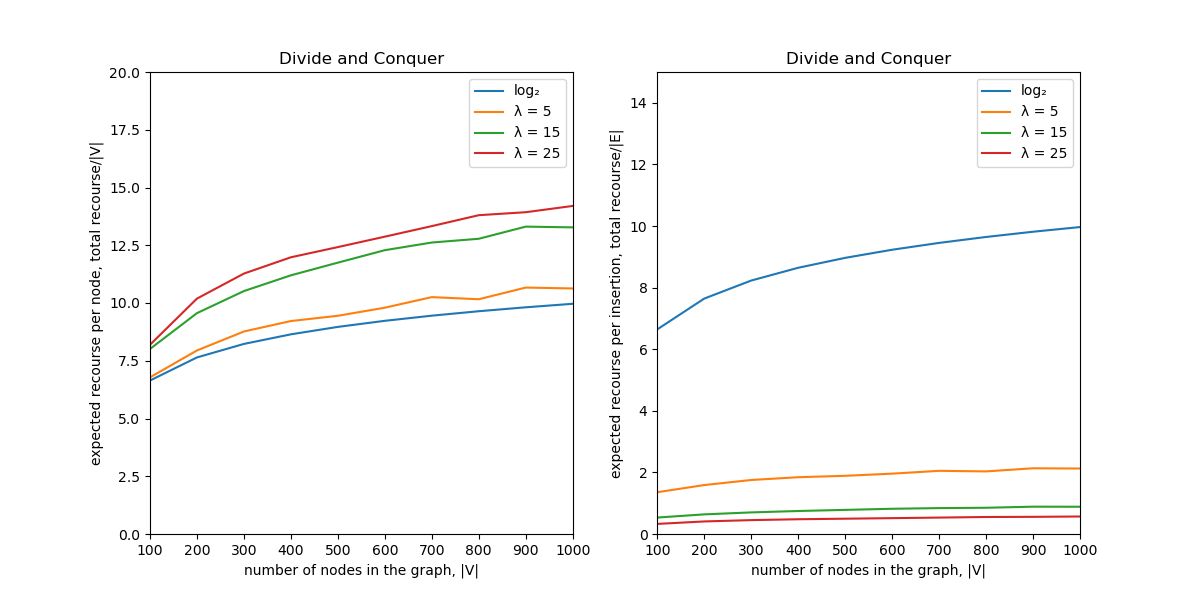
\includegraphics[width=18cm]{Images/DnCtests.png}}
    \caption{The curve $\lambda = k$ shows the average recourse of the divide and conquer algorithm per node (left) and per insertion (right) over many randomly generated insertion sequences of length exactly $\lambda n$ on randomly generated DAGs with $n$ nodes.}
    \label{fig:recoursetests2prog}
\end{figure}

\subsection{Activation Sequence Framework}

This next framework will involve the \textit{simple one-way search algorithm}, $\pazocal A_1$. My supervisor, Sayan Bhattacharya, has conjectured that this incremental topological ordering algorithm satisfies Conjecture \ref{aimconj}. With this conjecture in mind, I have been able to construct a framework which has lead to partial results and a proof of a strengthened version of Conjecture \ref{aimconj} restricted to trees instead of DAGs, where we do not require the edges to be inserted uniformly at random.

The one way search algorithm is defined as follows.

\begin{algorithm}[H]\label{oneway}
    \SetAlgoLined
    \KwIn{DAG $G=(V,E)$, a topological ordering $\prec$ of $G$, and an edge $e = (u,v) \notin E$ such that $G \cup \{e\}$ is a DAG}
    \KwOut{a topological ordering $\prec^*$ of $G \cup \{e\}$}
    
    \If{$u \prec v$}{return $\prec$\;}
    
    $\triangleright$ suppose $u_1 \prec ... \prec u_n$\;
    $\triangleright$ suppose $u = u_j$ and $v=u_i$ for some $1 \leq i < j \leq n$\;
    
    $S \leftarrow \varnothing$\;
    $k \leftarrow i$\;
    
    \While{$k \leq j$}{
        \If{$u_k \in reach_G(v)$}{
            $S.push(u_k)$\;
        }
        $k \leftarrow k+1$\;
    }
    
    \While{$S \neq \varnothing$}{
        $x \leftarrow S.pop()$\;
        move $x$ just to the right of $u$ in $\prec$\;
    }
    return $\prec$\;
    \caption{The Simple One-Way Search Algorithm, $\pazocal A_1$}
\end{algorithm}

Let $G=(V,E)$ be a DAG. We call that orderings of the edges in $E$ the \textit{insertion sequences} of $G$, and denote the set of all insertion sequences of $G$ by $\mathcal S_E$. Similarly, we denote the set of all orderings of $V$ by $\mathcal S_V$. For some fixed insertion sequence and some $u \in V$, let $reach_t(u)$ and $reach_t^{-1}(u)$ be the set of all descendants and ancestors of $u$ respectively after the first $t$ edges have been inserted into the graph. 

I was able to prove that when we are considering the recourse of $\pazocal A_1$ on some input, we can assume without loss of generality that the graph contains some root node $r$ such that every other node in the graph is an ancestor of this node. Using this fact I came up with the following definitions.

Let $G=(V,E)$ be a DAG with root $r$.

\begin{definition}[Node Activation]
Given some $u \in V$ and an insertion sequence $\pazocal E$ of $G$, we say that $u$ is \textbf{activated} at time $t$, if $u \in reach^{-1}_t(r)$ and $u \notin reach^{-1}_{t-1}(r)$.
\end{definition}

\begin{definition}[Activation Sequence]
Let $\pazocal E$ be any insertion sequence of $G$. The \textbf{activation sequence} of $\pazocal E$, denoted by $\alpha = act(\pazocal E)$, is a sequence of length $m$ of potentially empty sets that form a partition of $V$, where $\alpha_t$ is the set of nodes activated at time $t$ and $\alpha_0 = \{r\}$.
\end{definition}

Here, the set $\alpha_t \subseteq V$ is the set of nodes that are able to reach $r$ for the first time after the insertion of $\pazocal E_t$. We can see that $act(\pazocal E)$ depends only on the graph and the insertion sequence, not the initial ordering. We now make a simple but useful observation about activation sequences.

\begin{definition}\label{gammafunction}
Let $\Gamma : act_r(\mathcal{S}_{E}) \times \mathcal S_V \longrightarrow \mathbb{N}$ be a map such that given some insertion sequence $\pazocal E$ of $G$ with activation sequence $\alpha$ and an ordering $\prec$ of $V$, $\Gamma(act(\pazocal E), \prec)$ is the length of the sequence of nodes $(u_j)_{j=1}^k$ defined recursively by
\[ u_0 = r, \;\;\; u_i \in \alpha_{\phi_i},\forall u \in \alpha_{\phi_i}, u \preceq u_i \]
\[ \phi_0 = 0, \;\;\; \phi_{i+1} = min\{j : \exists u \in \alpha_j, u_i \prec u, \phi_i < j\}\]
\end{definition}

Using these definitions, I was able to prove that if $G$ is a tree, then for some initial ordering of the nodes $\prec$, and insertion sequence $\pazocal E$, we have that $\Gamma(act(\pazocal E), \prec)$ is exactly the recourse of $\pazocal A_1$ on this input. Since I was also able to show that by generating the initial ordering $\prec$ uniformly at random we get the expected value of $\Gamma(act(\pazocal E), \prec)$ is $\pazocal O(\log n)$ for any insertion sequence $\pazocal E$, we get that for any insertion sequence, as long as we start with a random ordering, we expect the recourse of $\pazocal A_1$ to be $\pazocal O(n \log n)$ since we can apply this argument to each node in the graph individually.

\section{Schedule Accuracy}

So far, I have not encountered any issues or problems while working on this project. In fact, it has gone much better than anticipated, and I have been able to make significant progress with all the aspects of my project, leaving me months ahead of the schedule I described in Section \ref{timetable} of my original specification. 

\section{Next Stage}

As I have discussed with my supervisor, the work I have already done is sufficient for the survey aspect of my project. I will devote the rest of my time to working on extending the frameworks I have designed and coming up with new observations in order to try and solve the open problem I described above. If I am successful, I may also tackle a more difficult version of this problem, where we allow the edges to be inserted into the graph in any order. As I briefly covered above, I have already solved this in the case where the graph is a tree, and it may be possible to extend my activation sequence framework to all DAGs if I am able to establish a relationship between values of $\Gamma$ and the recourse of $\pazocal A_1$. 

% \section{Objectives}

% The following is a outline of how I plan to structure my final report. I may reorder the topics or present some of them at the same time depending on what is more natural.

% \begin{enumerate}
%     \item Introduce the problem in both an intuitive and formal way while introducing relevant notation. ($\approx$ 1 - 2 pages)
    
%     \item Briefly survey the current state of the problem. Such as going over how the problem is \textit{well understood} for dense graphs but not for sparse graphs, and giving some of the more important results in the area. ($\approx$ 2 - 3 pages)
    
%     \item Give descriptions of various algorithms that solve the problem efficiently, explaining their fundamental ideas at a high level without giving pseudocode, but still formally stating important Lemmas and Theorems and outlining their proofs in a clear and intuitive way. ($\approx$ 6 - 8 pages)
    
%     [ - Everything past this point will be my work on the problem - ]
    
%     \item Introduce the notion of the \textit{recourse} of an algorithm here, explaining why it's interesting and relevant. Simultaneously introduce the \textit{simple one-way search algorithm} $\pazocal A_1$ and the \textit{simple greedy two-way search algorithm} $\pazocal A_2$. Then introduce the random order arrival model, and the conjectures that $\pazocal A_1$ and $\pazocal A_2$ have low recourse under random order arrival. ($\approx$ 1 - 2 pages)
    
%     \item I may introduce my framework for divide and conquer incremental topological ordering algorithms here, depending on how well it fits and if I think it's interesting enough. ($\approx$ 5 - 6 pages)
    
%     \item Give my proof that $\pazocal A_2$ obtains $\pazocal O(n \sqrt m)$ recourse under adversarial arrival, then give the graph from [HKMST] that yields $\Omega(n \sqrt m)$ recourse on all local algorithms under adversarial arrival, followed by my detailed analysis that shows how this is does not hold under random order arrival. ($\approx$ 4 - 6 pages)
    
%     \item Give my Lemmas about the properties of $\pazocal A_1$, introduce my notion of \textit{activation sequences}, and using my Propositions and Lemmas prove that the expected total recourse of trees under adversarial arrival is $\pazocal O(n \log n)$ with expectation taken over initial orderings. ($\approx$ 4 - 6 pages)
    
%     \item Potentially go over a few of the many different ideas I had and things I tried while doing work on this problem. ($\approx$ 1 - 2 pages)
% \end{enumerate}

% If I have any new ideas these may change. I may also add some diagrams into some sections if I think it will be relevant. This current plan should be more than sufficient for the word count as it is.

\newpage

\appendix

\section{Project Specification}

\subsection{Problem}

Cycle detection in directed graphs is one of the classic problems studied in algorithmic graph theory. The problem is simple, given some directed graph $G$, does it contain a cycle? In this project I will be considering a dynamic version of this problem, where we are given a graph that initially has no edges (and hence no cycles) which is updated over time by a sequence of edge insertions. After each edge is inserted, we must return whether or not the updated graph is acyclic. This problem is referred to as \textit{incremental cycle detection}.

Suppose we have some DAG $G$ and we insert an edge into $G$ to obtain $G^{\star}$. It turns out that if we have access to a topological ordering $\prec$ of $G$, and we have an algorithm that we can use to compute a topological ordering $\prec^{\star}$ of $G^{\star}$ using $\prec$, then this can be used (with a small amount of overhead) to obtain an incremental cycle detection algorithm. Because of this, the problems of incremental cycle detection and \textit{incremental topological ordering} go hand in hand.

These are the two problems that I will be exploring throughout my project. I will be surveying the current state of the problems, going over the major results, describing state of the art algorithms, and trying to make my own observations along the way.

\subsection{Objectives}\label{objectives}

I have two main aims with this project. The first is to survey the problem of incremental cycle detection and topological ordering by reading and understanding the relevant literature on the topic. There are dozens of papers on this subject spanning several decades, but at their core, many of the algorithms and approaches in these papers rely on the same ideas. I plan on going over some of these ideas, giving descriptions of various algorithms that solve the problem efficiently, explaining their fundamental ideas at a high level but still formally stating important Lemmas and Theorems and outlining their proofs in a clear and intuitive way.

My second aim is to try and make some original observations as I go through and survey the papers. Ideally I would like to create a new candidate framework to solve the problem, use it to design an algorithm, and test some metrics on this algorithm, seeing how they compare to some of the other algorithms in the literature. After talking with my supervisor, I am also aware that there are various open problems related to this topic, mainly focused on obtaining ploy-log amortized update time or poly-log amortized \textit{recourse}, a metric related to update time, in certain settings. It may be interesting to look into this and consider certain settings, such as the \textit{random order arrival model}. However, it is likely that this is outside the scope of this project.

\subsection{Methodology}

I will first go about my project by reading some of the core papers on the topic, such as \cite{HaeuplerKMST12} and \cite{BenderFG09}, to start developing my intuition and understanding of the topic, seeing what types of arguments are used to solve the problem. I will then read some of the newer papers on the problem, such as \cite{BenderFGT16}, \cite{BernsteinC18} and \cite{BhattacharyaK20}, and compare them to the algorithms that I have already understood and interpreted, extracting the core ideas from them. Throughout this whole process I will be thinking about how the notions presented in the papers can me modified and extended in order to tackle some of the open questions in the area that I briefly mentioned before. I plan on having regular (weekly) discussions with my supervisor about the literature that I go through, as well as any ideas that I come up with.

\subsection{Timetable}\label{timetable}

As I have discussed with my supervisor, due to the many important responsibilities that I will have over the next few months, I am not able to come up with a very detailed timetable that I will be following at this moment. However, I have already started reading the papers and plan to have read through most of them by the end of this term. I will write up any observations that I make, as well as my interpretations of the algorithms, as I read through the papers. This will hopefully make it easy to produce the final report (and the progress report) once I have finished going through everything and have a good understanding of the problem. I plan on having the bulk of the project done by the end of February, leaving me time to focus purely on doing my own research on the problem to see if I can make some original observations or develop any ideas that I come up with while reading through the papers. If any delays do occur, it may reduce the amount of time that I have to do my own research on the problem, but this is not essential to the project so it should not cause any real problems.

The following dates are the deadlines that I will be meeting with the different parts of my project. As I work on the project this list will be expanded with more detailed objectives and dates.

\begin{flushleft}
    Term 1
    \newline
    
    24$^{th}$ Oct. Finish reading through 1 paper.
    
    7$^{th}$ Nov. Finish reading through 2 papers and making notes on 1 paper.
    
    21$^{th}$ Nov. Finish reading through 3 papers and making notes on 2 papers.
    
    23$^{th}$ Nov. Decide on some parts of the problem I want to try and expand on.
    
    25$^{th}$ Nov. Finish the progress report.
    
    5$^{th}$ Dec. Finish reading through 4 papers and making notes on 3 papers.
    \newline
    
    Term 2
    \newline
    
    16$^{th}$ Jan. Finish reading through all the papers and making notes on them.
    
    17$^{th}$ Jan. Start doing my own research on the problem.
    
    15$^{th}$ Mar. Finish preparing the presentation.
    
    11$^{th}$ Apr. Finish the first draft of the final report.
    
    1$^{st}$ May. Finish the final report.
\end{flushleft}

\subsection{Resources}

Being a mostly theoretical research project I will not need any resources that aren't readily available to most students. I only need access to Python and Java to run code and carry out some tests.

\subsection{Legal, Social and Ethical and Issues}

Being a mostly theoretical research project that will not involve working with people apart from my supervisor, I did not not need to consider any legal, social or ethical issues.

\newpage

\bibliographystyle{alpha}
\bibliography{refs}

\end{document}